\section{TP3 : Transmission bruitée analogique (bruit blanc gaussien)}
\sectionmark{TP3 : Transmission bruitée analogique (bruit blanc gaussien)}

\subsection{Introduction étape 3}

Dans la continuité des étapes 1 et 2, l’objectif principal de cette simulation est d'étudier le comportement du système de transmission lui-même. Cette fois-ci, on prendra en compte une transmission non-idéale avec canal bruité de type \textit{gaussien}. La propagation dans le canal est modélisée de manière théorique par un bruit blanc additif gaussien (AWGN - \textit{Additive white Gaussian noise}) qu’il conviendra de régler en fonction des paramètres du transmetteur vus à l’étape précédente.  


\subsection{Attendus}

Jusqu'alors nous avons implémenté une chaîne de transmission composée d'éléments analogiques et logiques, avec des CAN (Convertisseurs Analogique Numérique) modélisant les codages NRZ, NRZT et RZ. Chaque élément de cette chaîne est dit \textit{parfait}, c'est à dire que la transmission est idéale, sans perte (TEB à 0\%) et sans notion de bruit. Cette étape consistera donc à implémenter du bruit blanc gaussien au niveau du transmetteur, pour modéliser un comportement plus proche de la réalité. Cette section aura vocation à présenter les éléments pris en compte, leur implémentation dans le logiciel et une interprétation physique des résultats obtenus.

Pour apercevoir ces nouvelles implémentations, il faudra utiliser l'option suivante :

Le paramètre \texttt{-snrpb s} permet l'utilisation d’une transmission analogique bruitée, \texttt{s} est la valeur du rapport $\frac{Eb}{N0}$ (en dB). Le paramètre \texttt{s} doit être une valeur flottante. Par défaut, la transmission est non bruitée.

Java n'implémentant pas la loi gaussienne, il nous faudra implémenter celle-ci à partir de lois uniformes. Pour ce faire, nous utilisons la formule suivante :

\vspace{12pt}

$b(n)=\sigma_b\sqrt{-2ln(1-a_1(n))cos(2\pi a_2(n))}$; avec $a_1(n)$ et $a_2(n)$, des lois uniformes et $b(n)$ suivant une loi gaussienne. 

\vspace{12pt}

Dès lors, le signal de sortie sera donné par $s(n)=e(n)+b(n)$, avec $s(n)$ le signal de sortie, $e(n)$ le signal d'entrée et $b(n)$ le bruit blanc gaussien ajouté.

L'implémentation du rapport signal à bruit peut être obtenu de deux manières distinctes (toutes deux homogènes et semblables) :

\vspace{12pt}

\begin{itemize}
    \item $SNR=\frac{P_{signalE}}{P_{bruit}}$ ; Le rapport puissance moyenne du signal émis sur puissance moyenne du bruit.
    \item $\frac{E_b}{N_0}$ ; Le rapport de l'énergie binaire sur la densité spectrale moyenne de bruit.
\end{itemize}

\vspace{12pt}

C'est cette seconde solution qui sera implémentée dans le projet, celle-ci se portant mieux à un contexte de communication binaire. En effet, le rapport $\frac{E_b}{N_0}$ est particulièrement utile pour évaluer la performance des systèmes de communication numérique en termes de taux d'erreur binaire (TEB), celui-ci faisant intervenir la quantité d’échantillons par bit.

\begin{figure}[H]
    \centering
    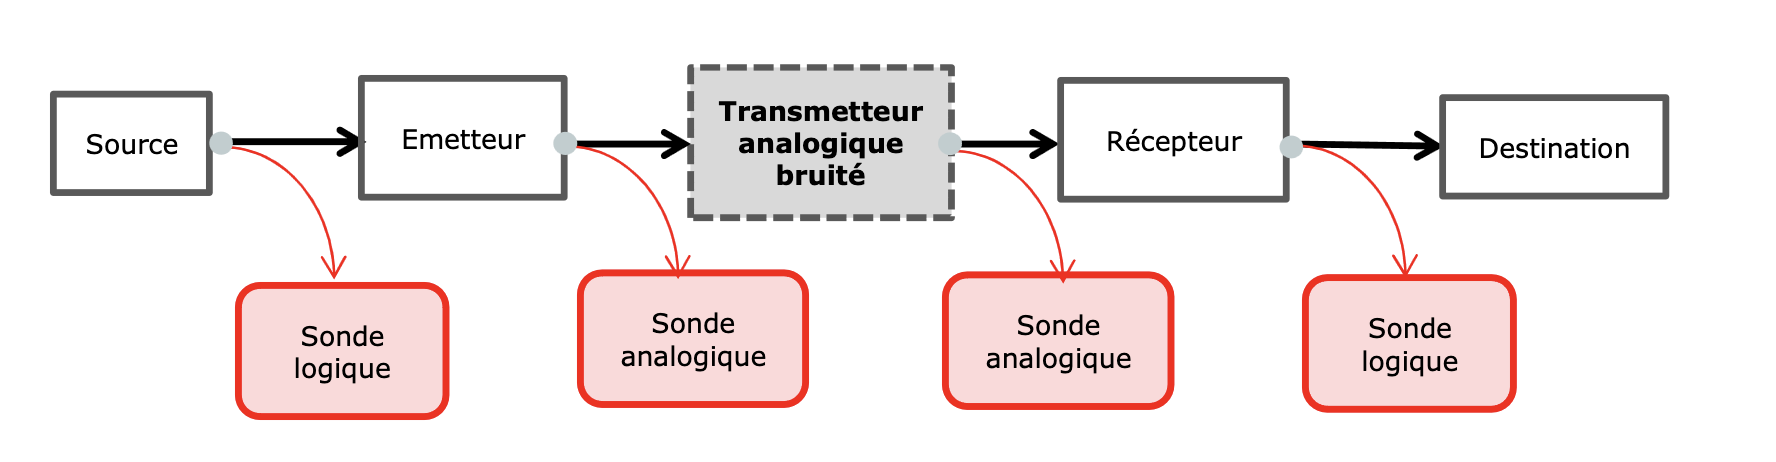
\includegraphics[width=0.9\textwidth]{img/etape2_chaine_transmission_bruitee.png}
    \caption{Chaîne de transmission bruitée}
    \label{fig:chaine_transmission_bruitee}
\end{figure}

\subsection{Réalisation}


\begin{figure}[H]
    \centering
    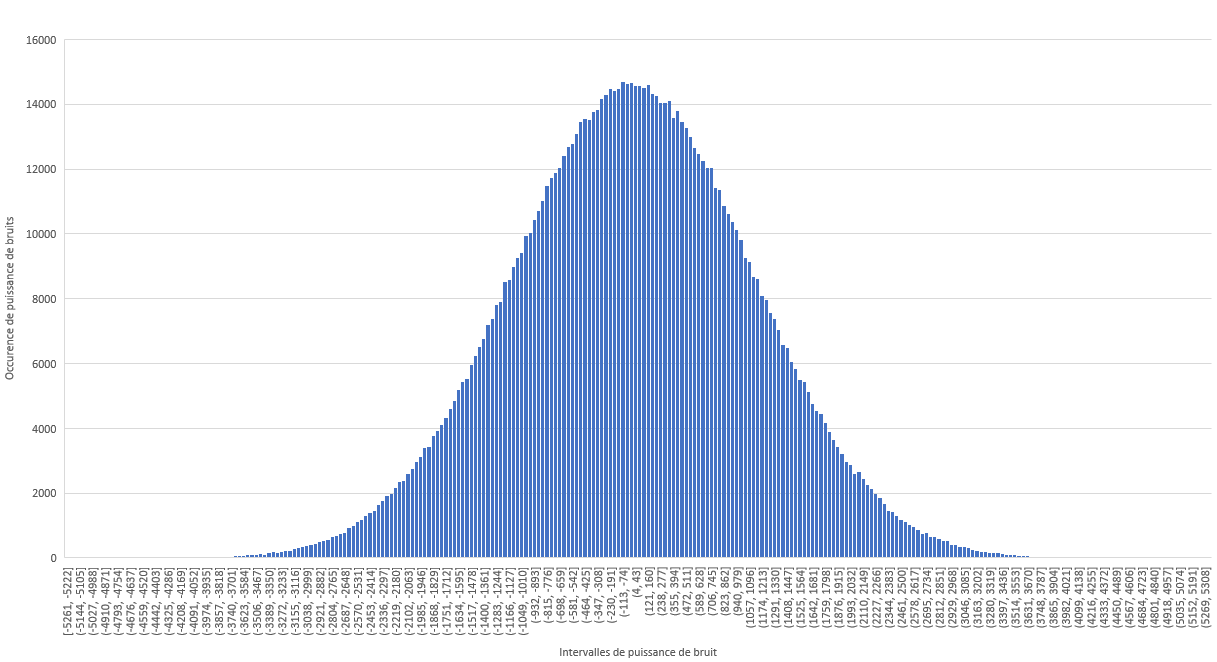
\includegraphics[width=\textwidth]{img/etape3_histo.png}
    \caption{Histogramme de la puissance de bruit moyenne pour 1 000 000 d'échantillons d'un message de 10 bits (NRZ)}
    \label{fig:etape3_histo}
\end{figure}

La répartition des valeurs sur la figure ci-dessus semble très nettement tendre vers une gaussienne (plus le nombre de valeurs sera important, et le pas entre les valeurs faible, plus la définition de cette gaussienne sera importante sur l'histogramme). 

La méthodologie à appliquer pour créer un signal bruité (signal blanc gaussien) étant désormais établie, nous pouvons nous focaliser sur sa mise en oeuvre. Pour cela les éléments suivants ont été implémenté :

Une classe java nommé \textbf{TransmetteurGaussien}, qui reprend le fonctionnement du \textbf{transmetteurParfait} et à laquelle on a ajouté trois méthodes:
     \begin{itemize}
        \item \texttt{calculerPuissanceMoyenneSignal()}
        \item \texttt{calculerVariance()}
        \item \texttt{genererSignalBruite()}
    \end{itemize}

\vspace{20pt}
   
Pour réaliser la méthode \texttt{calculerPuissanceMoyenneSignal()}, reprenons la formule théorique indiquant que la puissance du signal est égale à :

 \begin{align*}
    Ps = \frac{\sum_{i=1}^{k}S(n)^2}{k} 
 \end{align*}

 Nous avons besoin de la puissance du signal émis, pour calculer la valeur de la variance $\sigma_b^2$, car cette dernière nous permet de générer notre bruit en fonction du SNR. On peut obtenir la valeur en renversant l'équation:

\begin{align*}
   SNR =& \frac{P_s * N}{2\sigma b^2}\\
   \sigma_b^2 =& \frac{Ps*N}{2*10^{\frac{SNR}{10}}}\\
\end{align*}
en prenant N le nombre d'échantillon et Ps la puissance du signal

On obtient alors la valeur de $\sigma$:
\begin{align*}
 \sigma_b =& \sqrt{\frac{Ps*N}{2*10^{\frac{SNR}{10}}}}\\
\end{align*}

À partir de la valeur trouvé ci-dessous, on peut désormais générer notre bruit blanc gaussien pour réaliser le transmetteur bruité. Grâce à l'étape deux et aux calculs ci-dessus, on peut modéliser le passage d'un bruit blanc gaussien à travers différents types de codage (RZ, NRZ, NRZT) :

\subsubsection{Émission analogique RZ d'un signal bruité}
\begin{figure}[H]
    \centering
    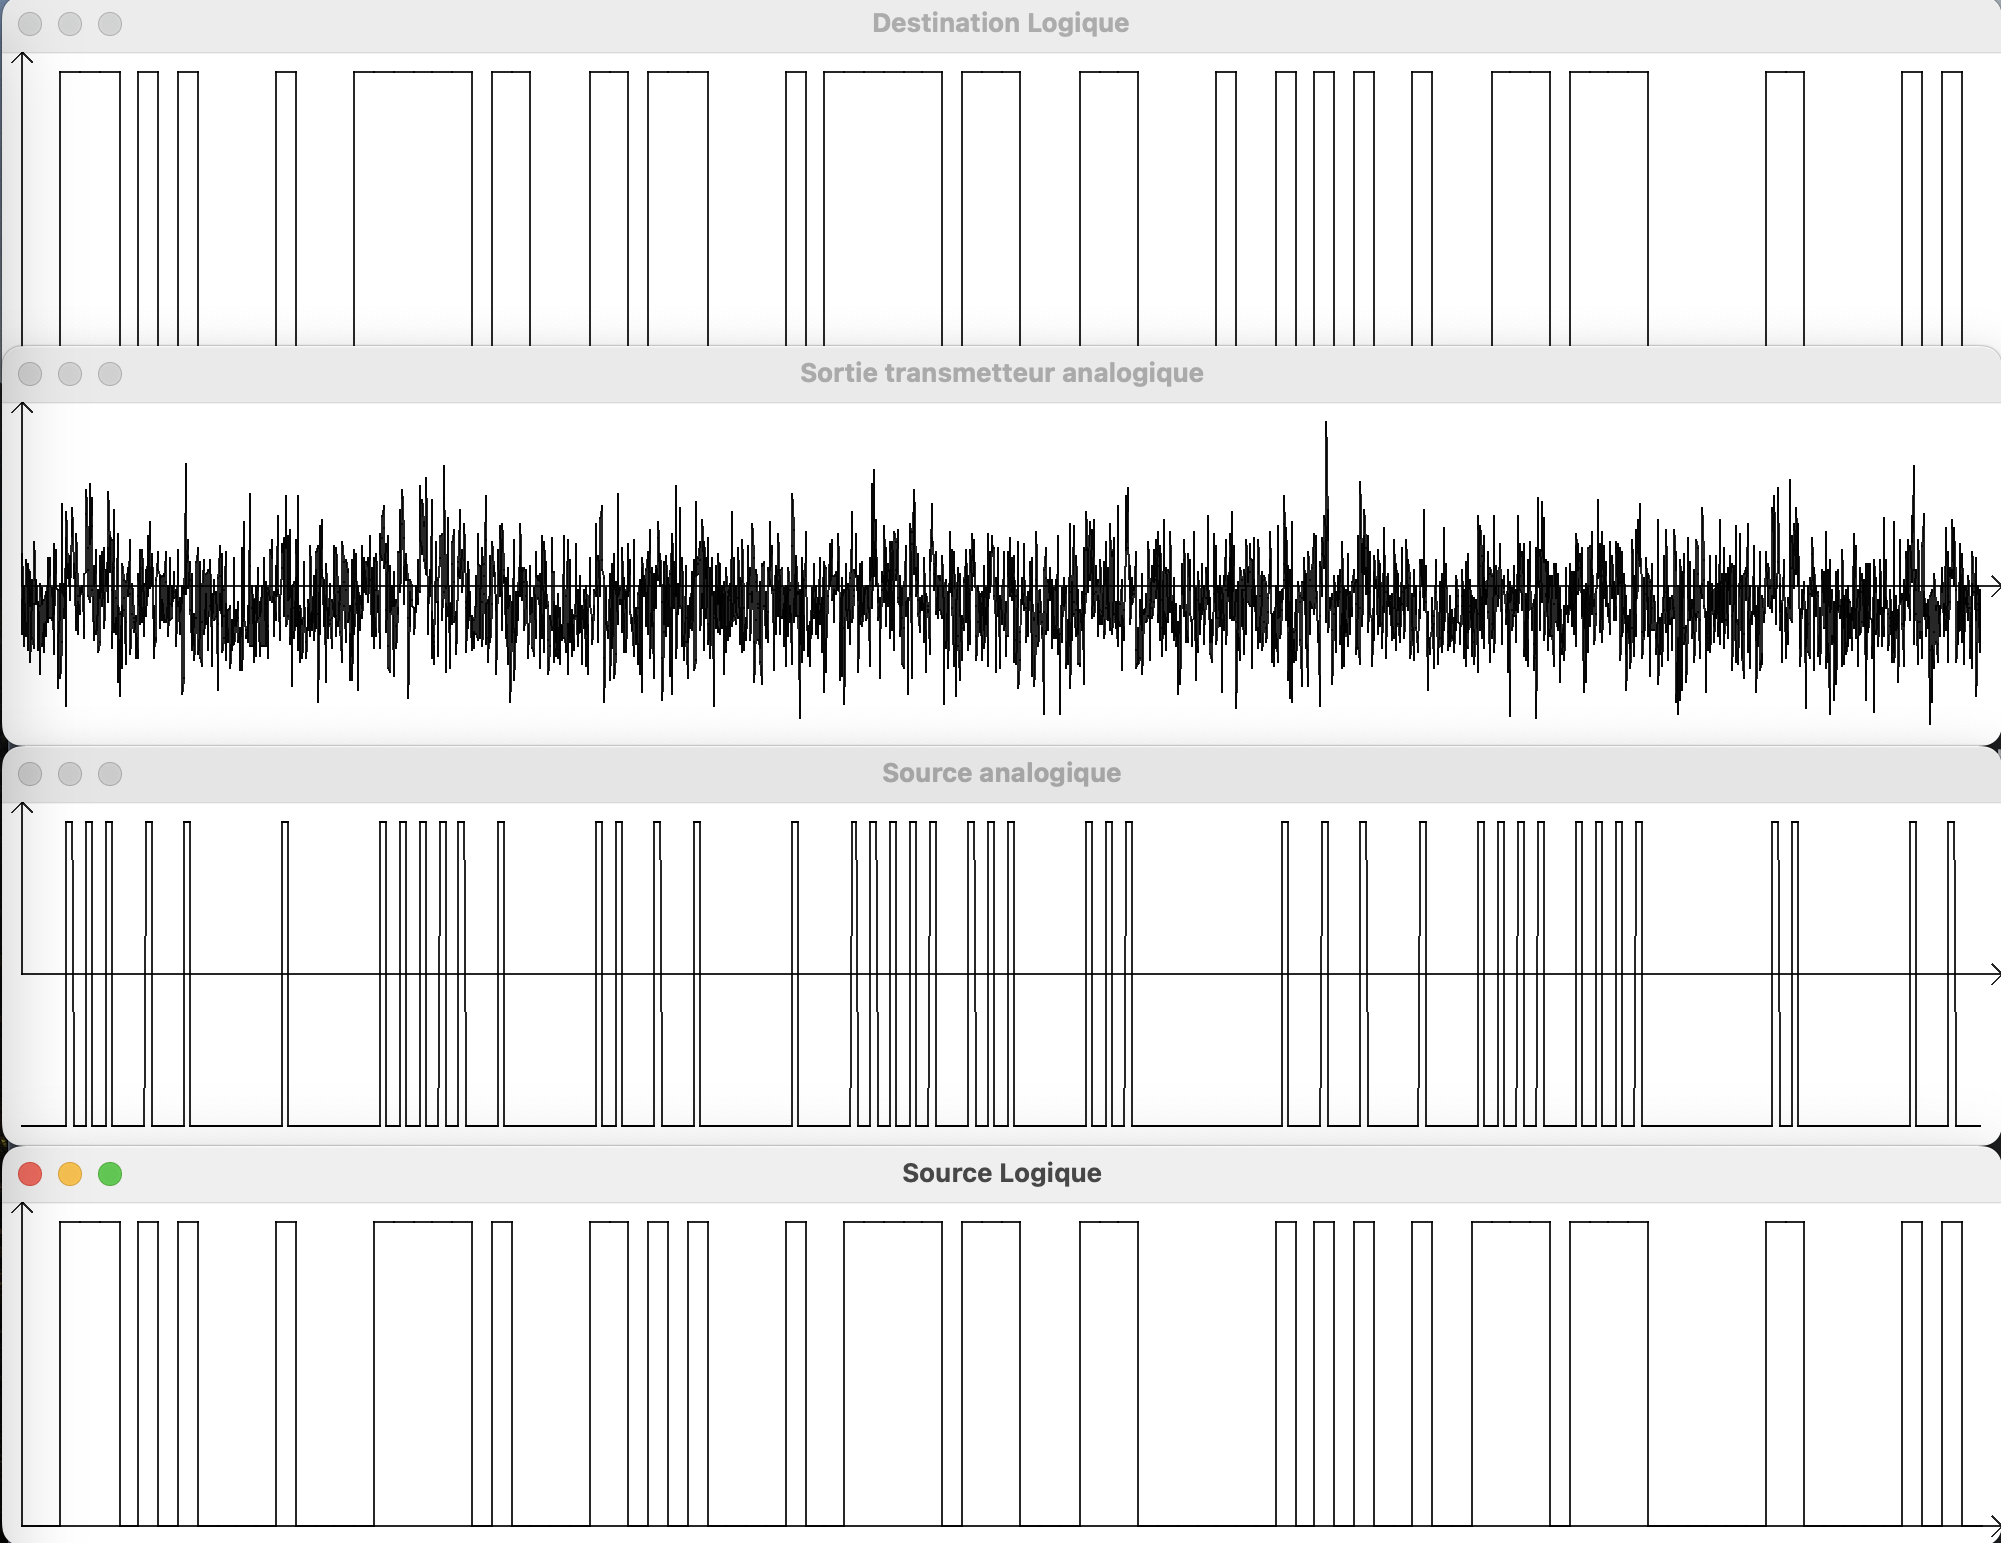
\includegraphics[width=0.7\textwidth]{img/etape3_emission_RZ_bruite.png}
    \caption{Graphe des sondes de la chaîne de transmission pour un message de 100 bits de forme RZ et pour un SNR de 5 }
    \label{fig:etape_3_RZ_bruite}
\end{figure}

On réalise la simulation d'un signal bruité RZ de 100 bits et un SNR de 5. D'après ce que l'on a déjà simulé à l'étape 2, on observe bien au niveau de la sonde pour l'émission analogique, chaque changement de valeur d'un bit logique est suivi d'un passage par l'état 0. Pour ce qui est du transmetteur bruité, on remarque très clairement l'ajout de bruit au signal d'origine. Cela va entraîner des erreurs à la sortie du transmetteur, on voit notre TEB a une valeur de 0.06.

\begin{figure}[H]
    \centering
    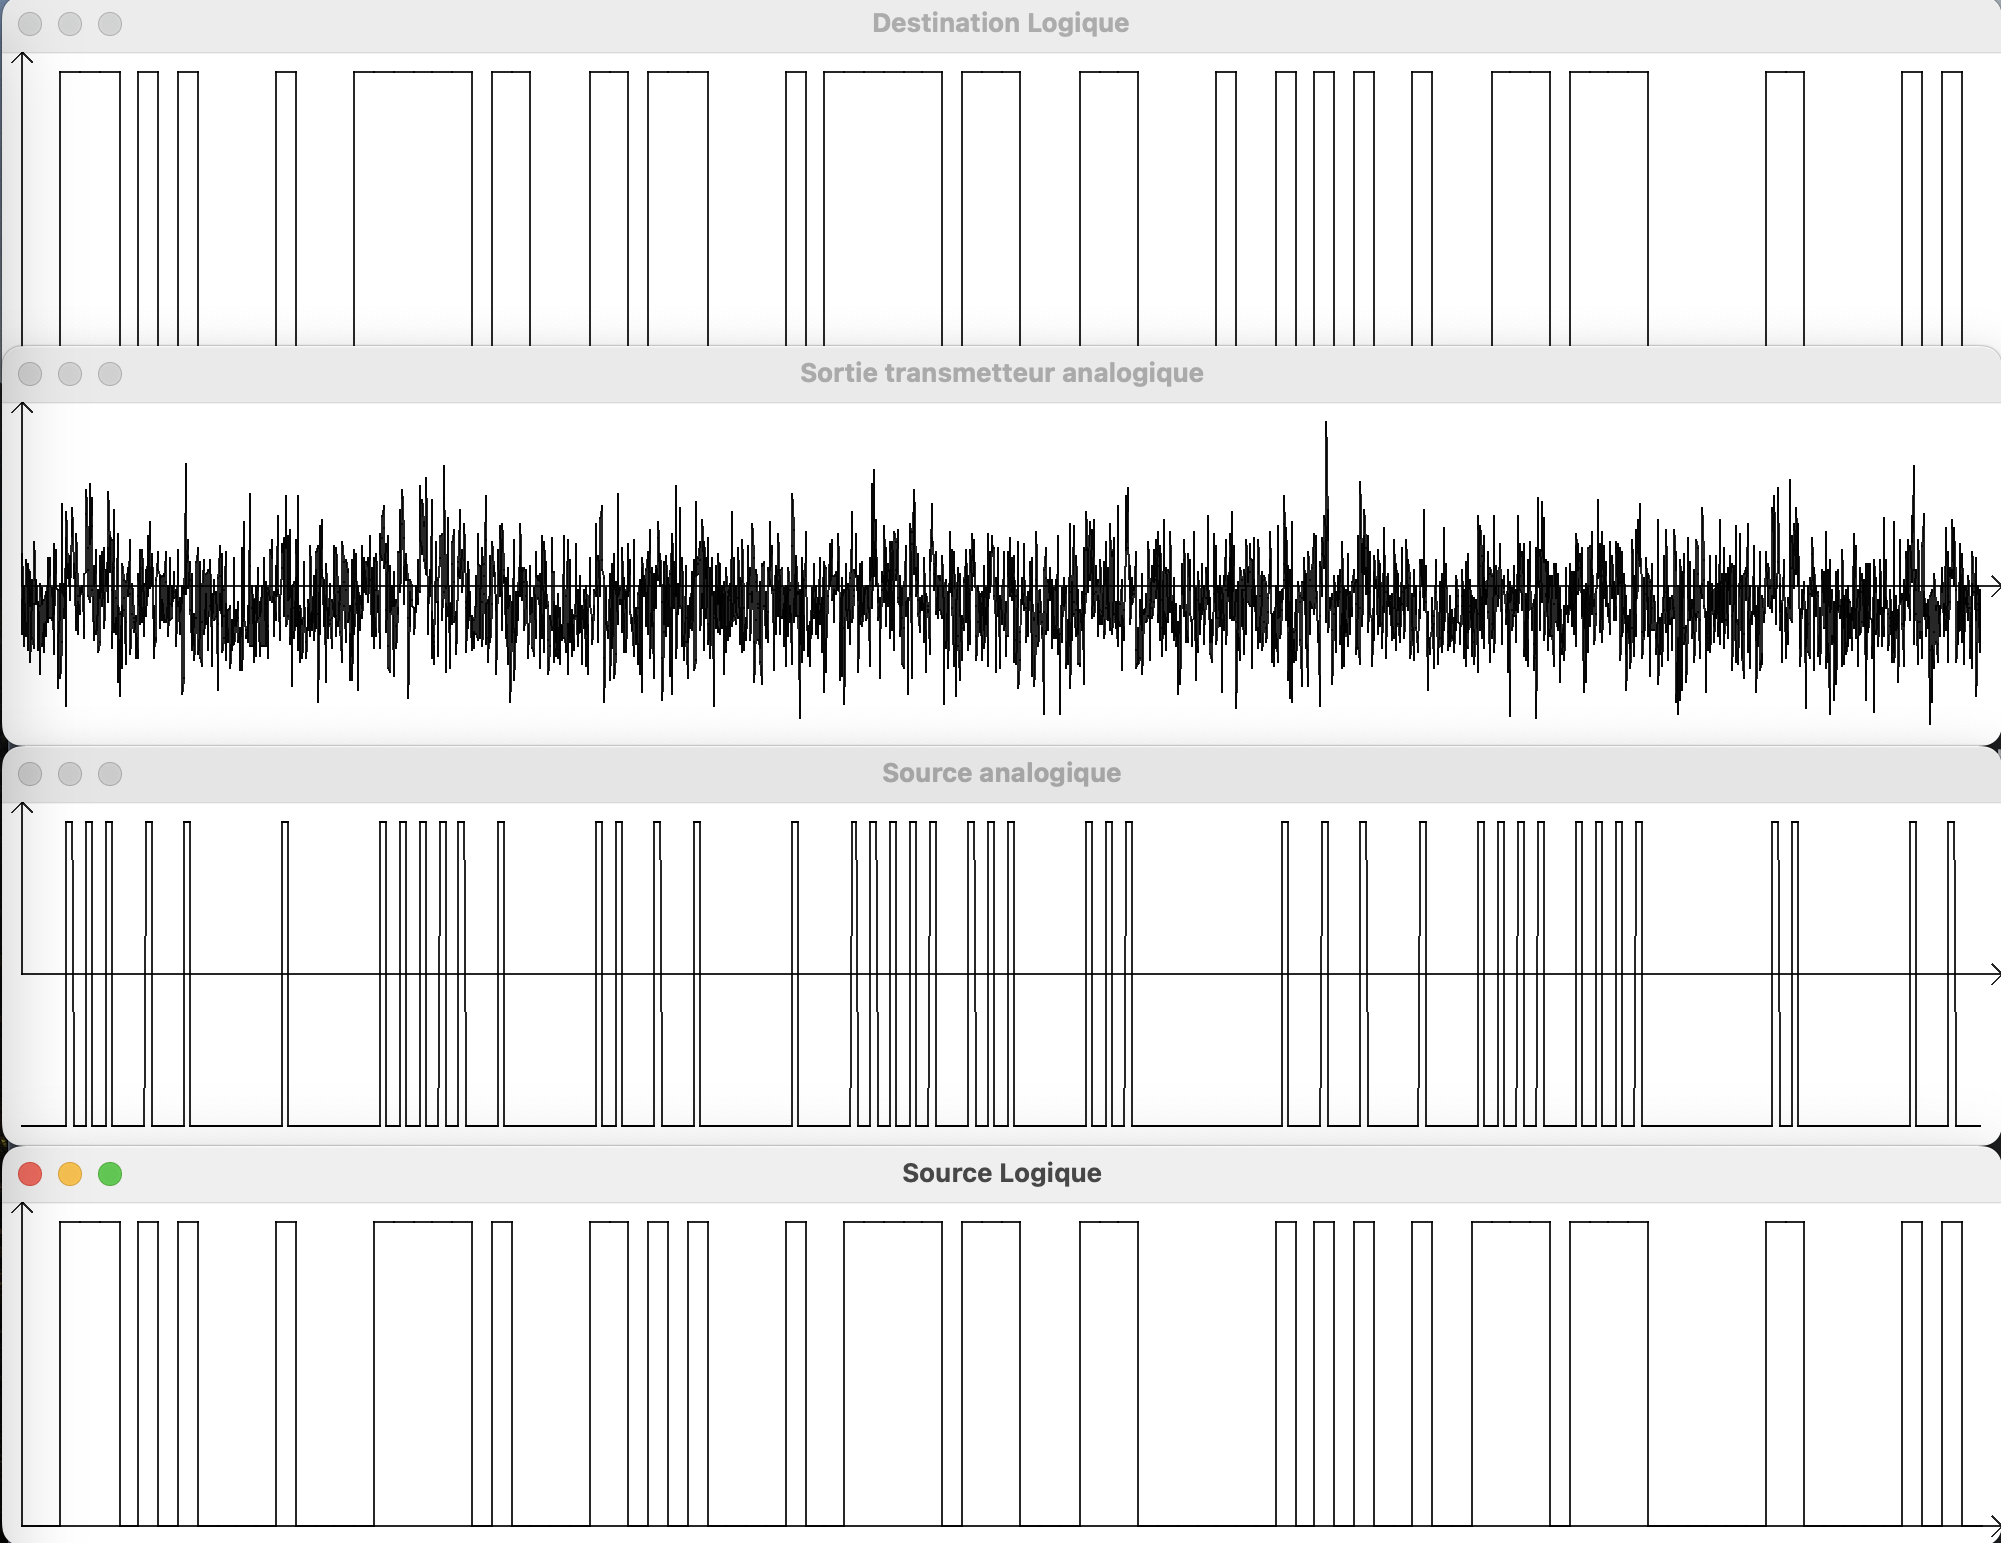
\includegraphics[width=0.7\textwidth]{img/etape3_emission_RZ_bruite.png}
    \caption{Graphe montrant l'évolution du TEB en fonction du SNR pour un signal RZ }
    \label{fig:etape_3_RZ_bruite}
\end{figure}

L'observation que l'on peut faire de ce graphe est que la valeur du TEB va tendre vers 0.5 lorsque l'on a une valeur de SNR augmente dans les négatifs. Au contraire lorsque le SNR augmente dans les positifs, la valeur du TEB diminue, et tend vers 0. Il y a une probabilité assez importante d'avoir une erreur de codage du signal.


\subsubsection{Émission analogique NRZ d'un signal bruité}

\begin{figure}[H]
    \centering
    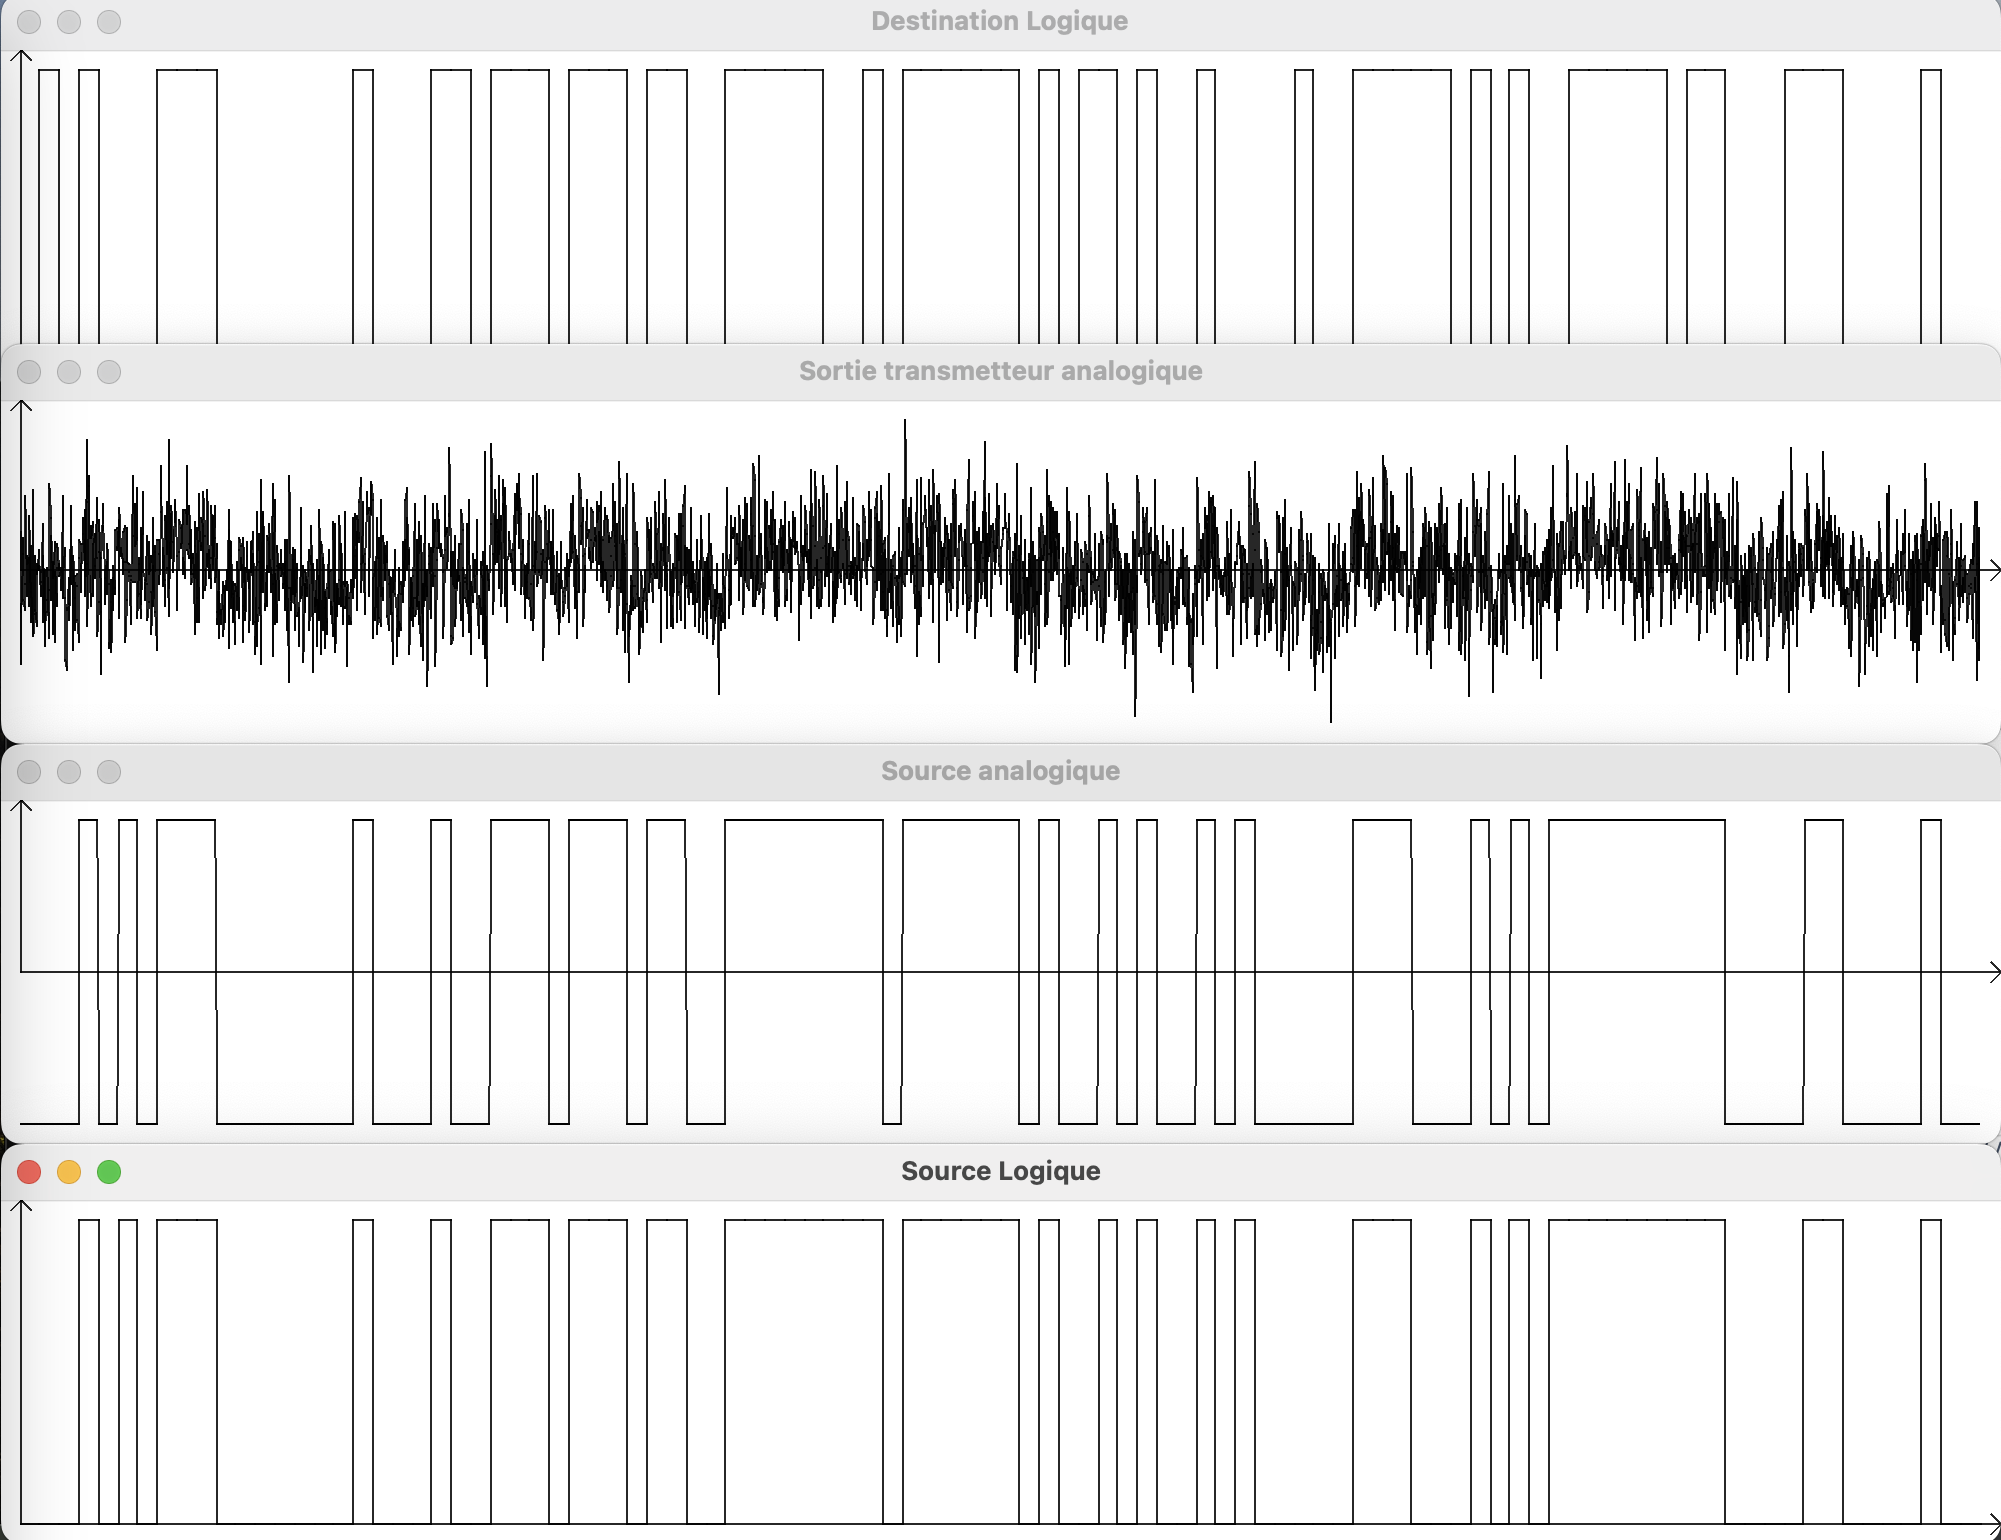
\includegraphics[width=0.7\textwidth]{img/etape3_emission_NRZ_bruite.png}
    \caption{Graphe des sondes de la chaîne de transmission pour un message de 100 bits de forme NRZ et pour un SNR de 5 db}
    \label{fig:etape_3_NRZ_bruite}
\end{figure}

On réalise la simulation d'un signal bruité NRZ de 100 bits et un SNR de 5. D'après ce que l'on a généré pour l'étape 2, on remarque bien les caractéristique du signal NRZ sur la simulation. En effet, on a bien un signal codé à l'aide de deux états, sans état intermédiaire. Pour ce qui est du transmetteur bruité, on remarque très clairement l'ajout de bruit au signal d'origine. Notamment, aux niveaux des amplitudes du signal, on observe une variation importante après l'ajout du bruit. C'est la cause de l'augmentation du TEB, l'ajout de bruit fait parfois dépasser le seuil de détection du symbole, ce qui peut empêcher la récupération du message côté récepteur. Ce phénomène est visible sur la simulation car on obtient un TEB de 0.19.

\begin{figure}[H]
    \centering
    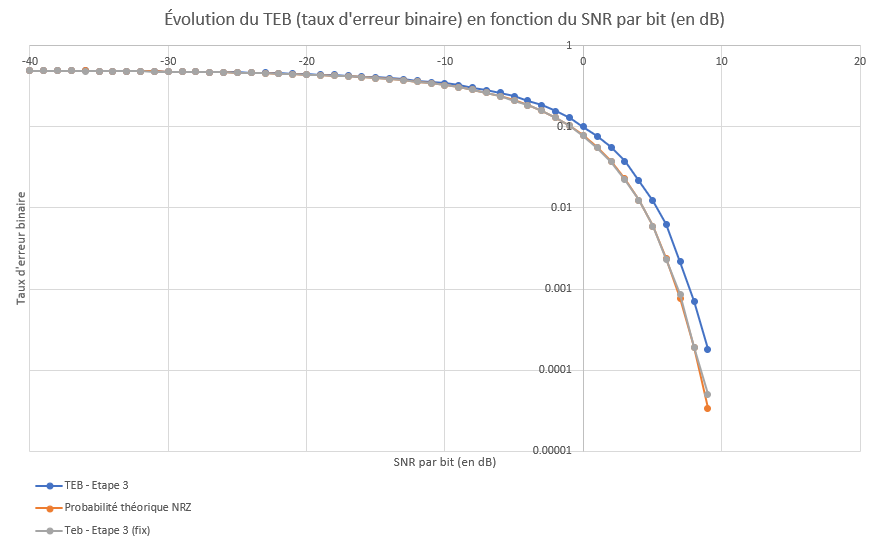
\includegraphics[width=0.8\textwidth]{img/etape3_teb_fct_snr.png}
    \caption{Tracé du TEB en fonction du SNR par bit (semence constante, message de 100000 symboles, codage NRZ, 30 échantillons par symbole)}
    \label{fig:etape3_teb_fct_snr}
\end{figure}

L'analyse de la courbe ci-dessus met en évidence une relation significative entre le rapport signal sur bruit ($\frac{E_B}{N_0}$) et le taux d'erreur binaire (TEB/BER). En effet, lorsque le rapport signal sur bruit est faible, le TEB augmente considérablement, ce qui reflète la sensibilité du signal à un environnement bruité. À l'inverse, lorsque le SNR est élevé, le bruit a moins d'impact, ce qui se traduit par une réduction du TEB. Il convient d'observer les courbes théoriques de chaque type de modulation et de les comparer aux résultats expérimentaux de notre système.

\subsubsection{Émission analogique NRZT d'un signal bruité}
\begin{figure}[H]
    \centering
    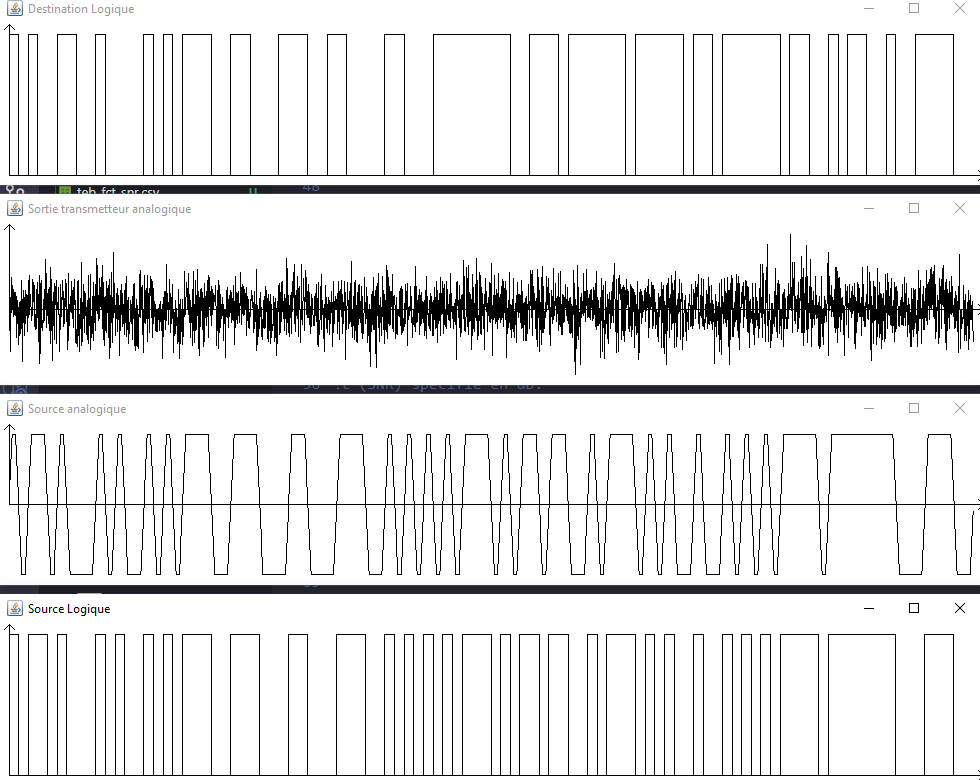
\includegraphics[width=0.7\textwidth]{img/etape3_emission_NRZT_bruite.png}
    \caption{Graphe des sondes de la chaîne de transmission pour un message de 100 bits de forme NRZT et pour un SNR de 5}
    \label{fig:etape_3_NRZT_bruite}
\end{figure}

On réalise la simulation d'un signal bruité NRZT de 100 bits et un SNR de 5. D'après ce que l'on a déjà simulé à l'étape 2, on observe bien au niveau de la sonde pour l'émission analogique, chaque changement de valeur d'un bit logique est réalisé de manière progressive, on voit bien une pente pour la montée et descente du symbole. Pour ce qui est du transmetteur bruité, on remarque très clairement l'ajout de bruit au signal d'origine. Cela va entraîner des erreurs à la sortie du transmetteur, on voit notre TEB a une valeur de 0.167.

\begin{figure}[H]
    \centering
    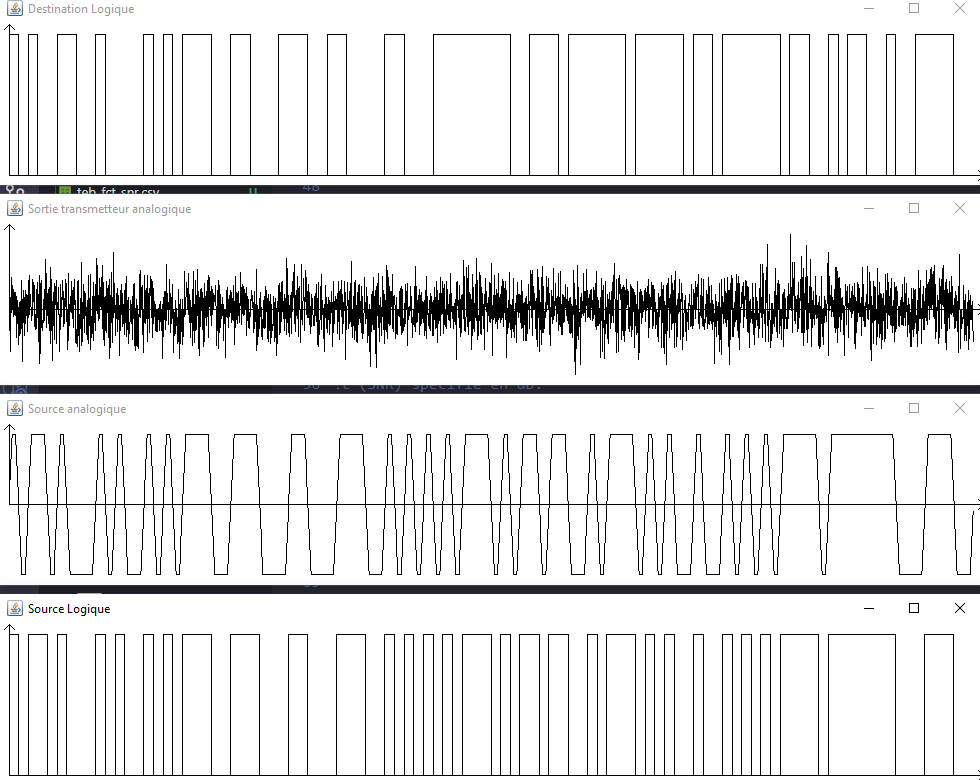
\includegraphics[width=0.7\textwidth]{img/etape3_emission_NRZT_bruite.png}
    \caption{Tracé du TEB en fonction du SNR par bit (semence constante, message de 100000 symboles, codage TNRZ, 30 échantillons par symbole)}
    \label{fig:etape_3_NRZT_bruite}
\end{figure}

L'analyse de la courbe ci-dessus met en évidence une relation significative entre le rapport signal sur bruit ($\frac{E_B}{N_0}$) et le taux d'erreur binaire (TEB/BER). En effet, lorsque le rapport signal sur bruit est faible, le TEB augmente considérablement, ce qui reflète la sensibilité du signal à un environnement bruité. À l'inverse, lorsque le SNR est élevé, le bruit a moins d'impact, ce qui se traduit par une réduction du TEB. Il convient d'observer les courbes théoriques de chaque type de modulation et de les comparer aux résultats expérimentaux de notre système.


\subsection{Conclusion étape 3}

En conclusion, nous avons réussi à introduire un élément essentiel à la modélisation d'une chaîne de transmission : un canal de transmission analogique bruité. Ce canal a été conçu pour simuler les conditions réelles auxquelles les signaux sont confrontés lors de leur transmission dans un environnement physique, pour lequel la modélisation sous forme de bruit blanc gaussien prend sens (théorème central limite). Le paramètre clé ici est le rapport signal sur bruit ($\frac{E_B}{N_0}$), qui joue un rôle déterminant dans la qualité de la transmission.